\chapter{Anhang}\label{Anhang}
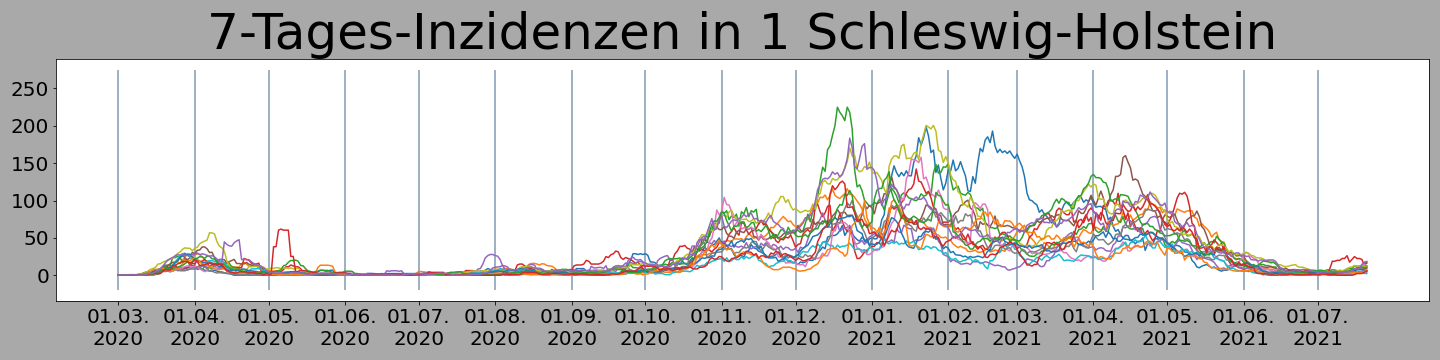
\includegraphics[width=\textwidth]{figures/Anhang/1_Schleswig-Holstein.png}
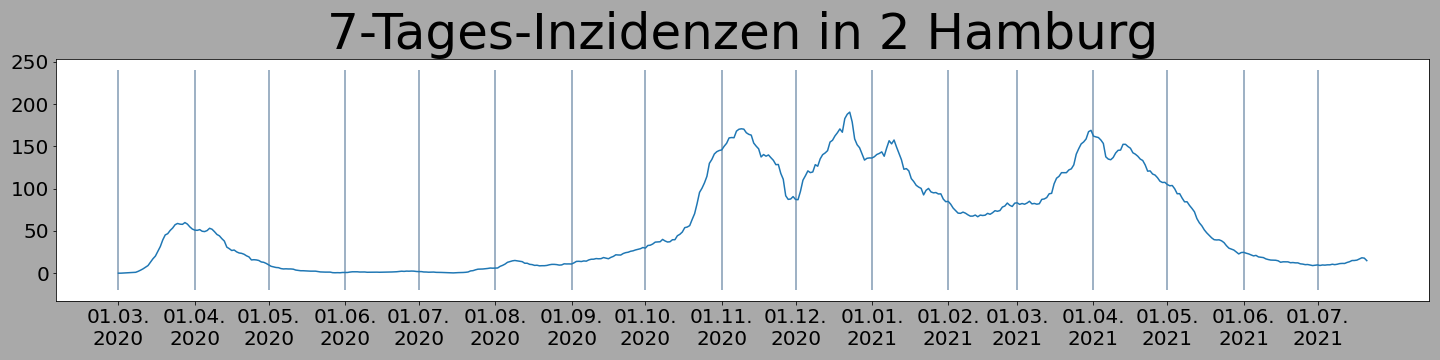
\includegraphics[width=\textwidth]{figures/Anhang/2_Hamburg.png}
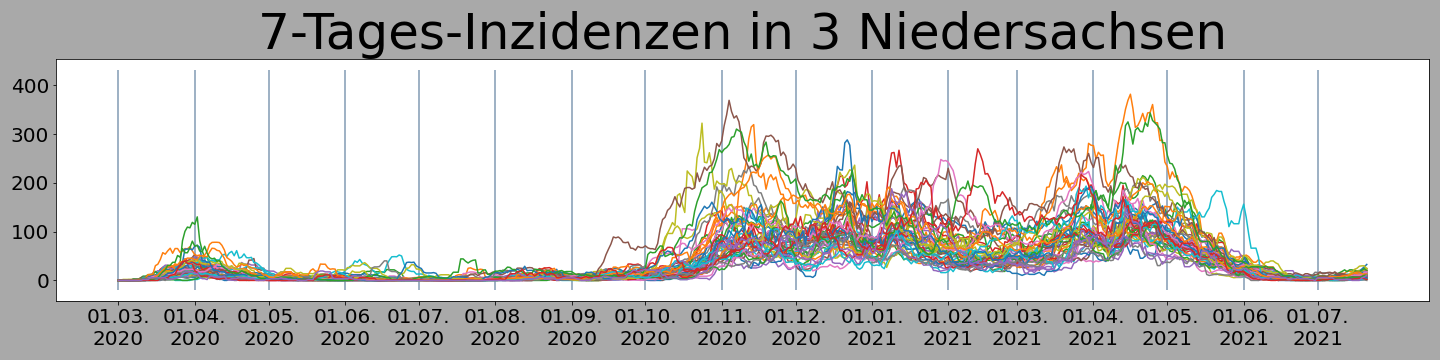
\includegraphics[width=\textwidth]{figures/Anhang/3_Niedersachsen.png}
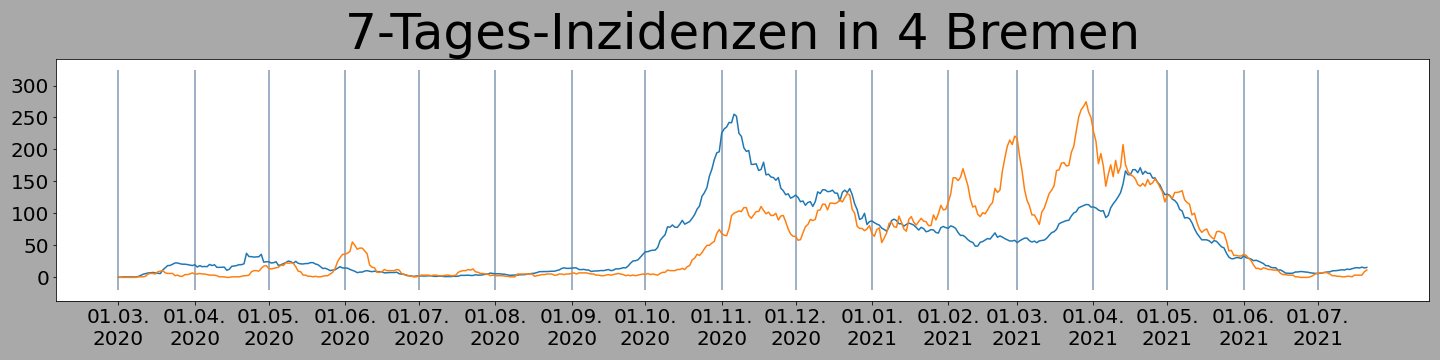
\includegraphics[width=\textwidth]{figures/Anhang/4_Bremen.png}
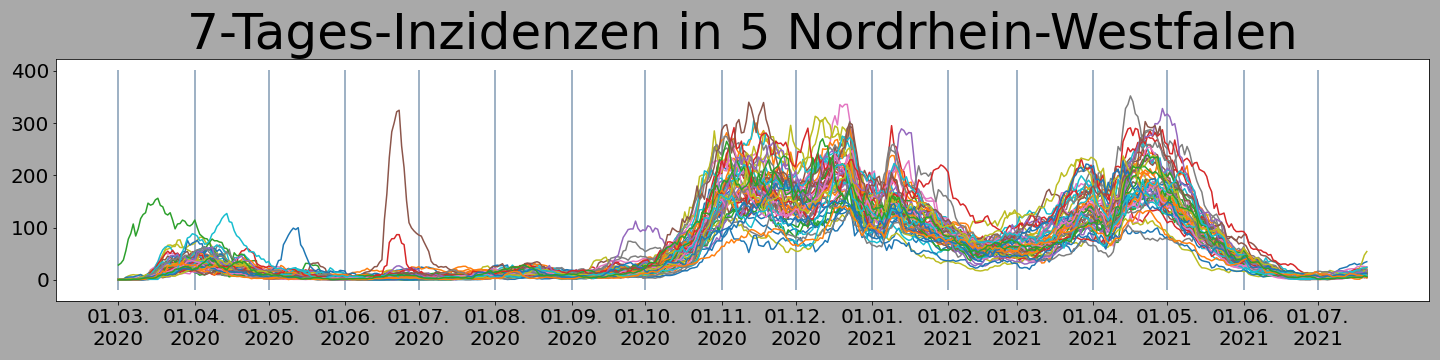
\includegraphics[width=\textwidth]{figures/Anhang/5_Nordrhein-Westfalen.png}
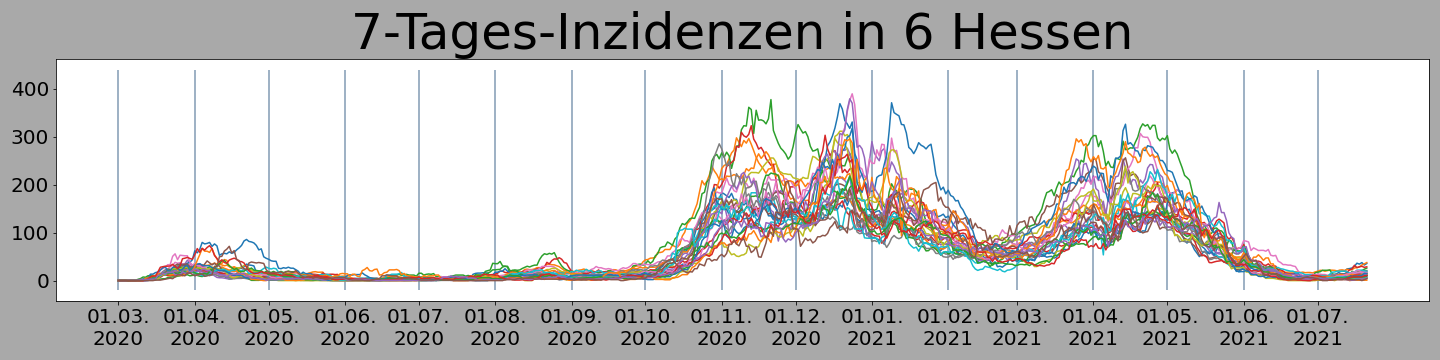
\includegraphics[width=\textwidth]{figures/Anhang/6_Hessen.png}
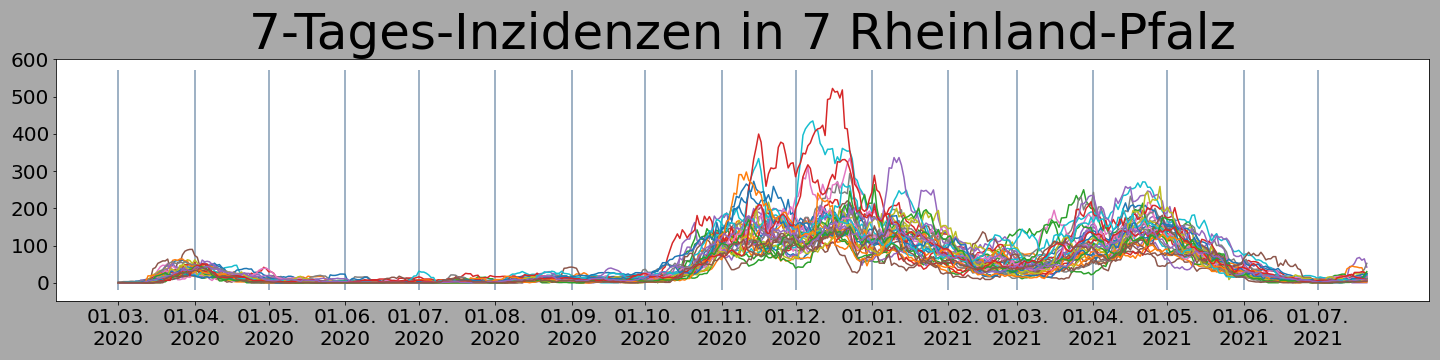
\includegraphics[width=\textwidth]{figures/Anhang/7_Rheinland-Pfalz.png}
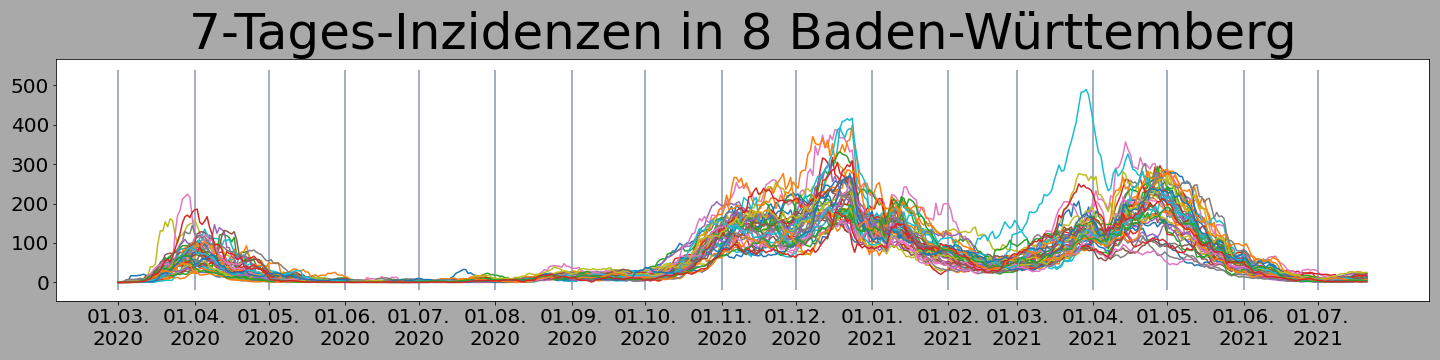
\includegraphics[width=\textwidth]{figures/Anhang/8_Baden-Württemberg.png}
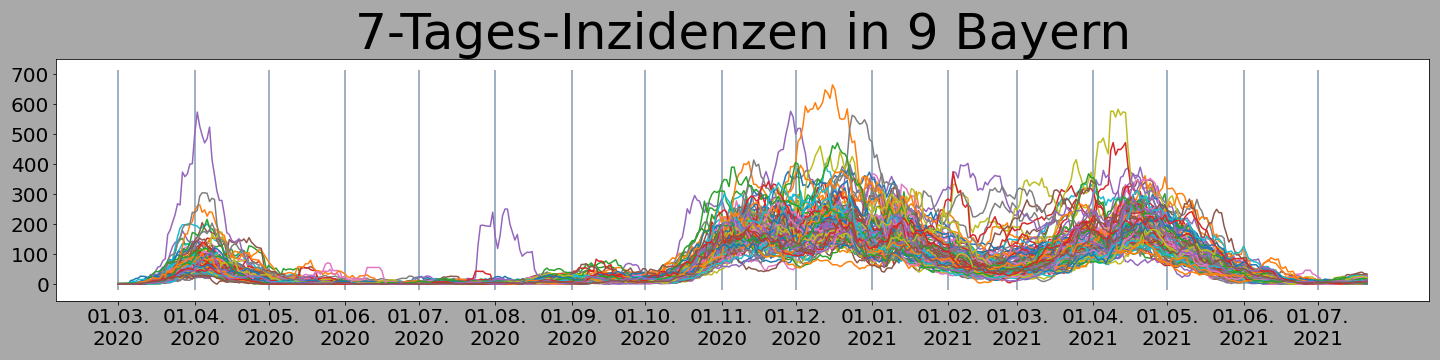
\includegraphics[width=\textwidth]{figures/Anhang/9_Bayern.png}
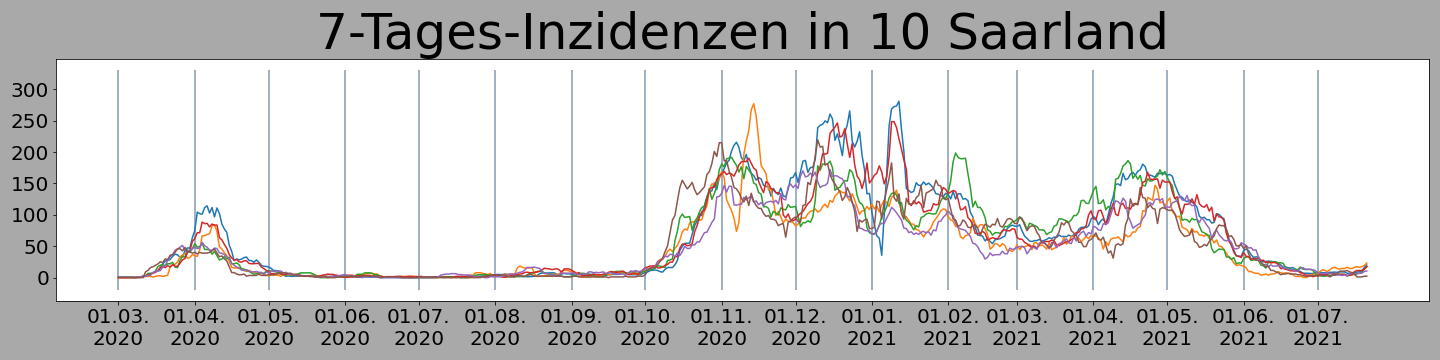
\includegraphics[width=\textwidth]{figures/Anhang/10_Saarland.png}
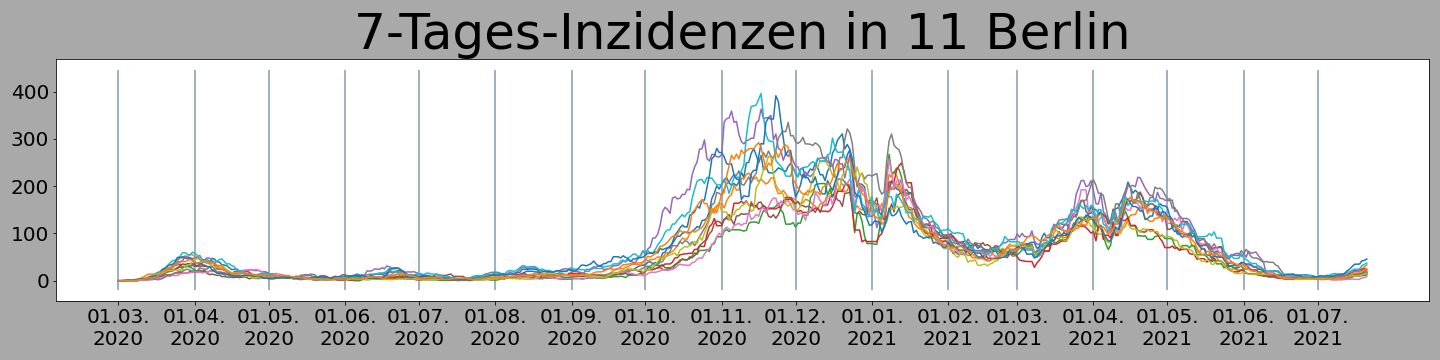
\includegraphics[width=\textwidth]{figures/Anhang/11_Berlin.png}
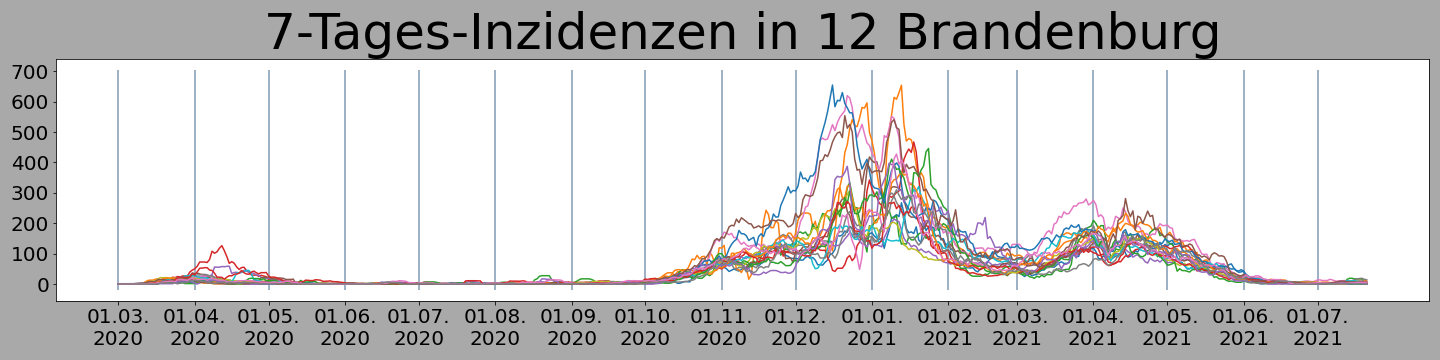
\includegraphics[width=\textwidth]{figures/Anhang/12_Brandenburg.png}
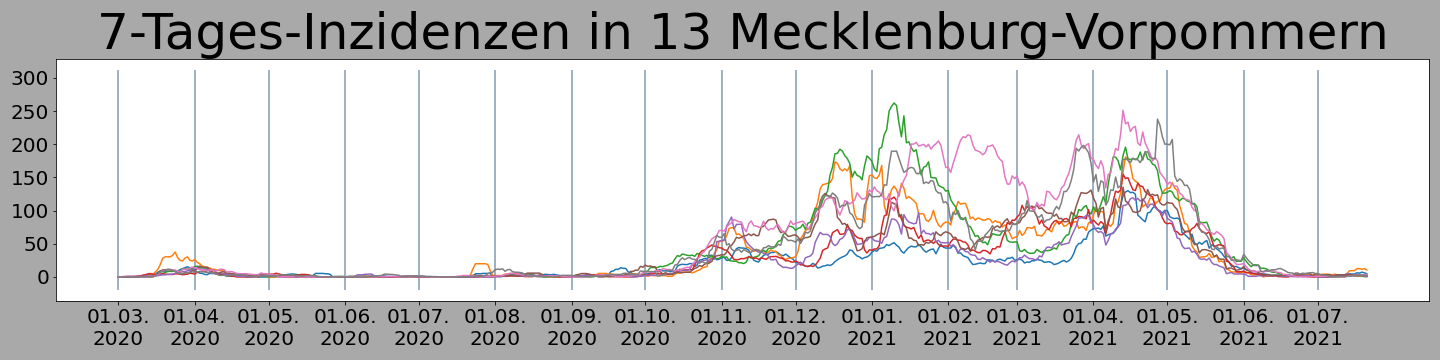
\includegraphics[width=\textwidth]{figures/Anhang/13_Mecklenburg-Vorpommern.png}
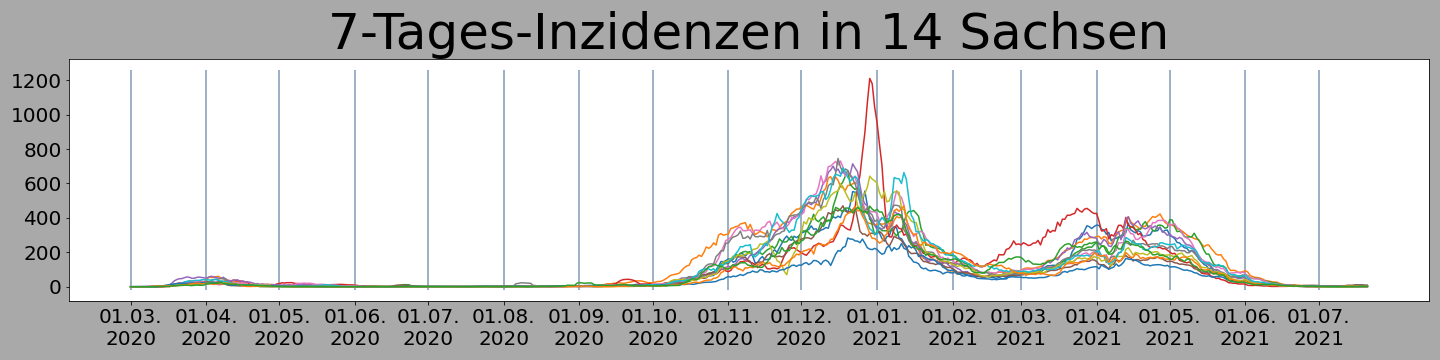
\includegraphics[width=\textwidth]{figures/Anhang/14_Sachsen.png}
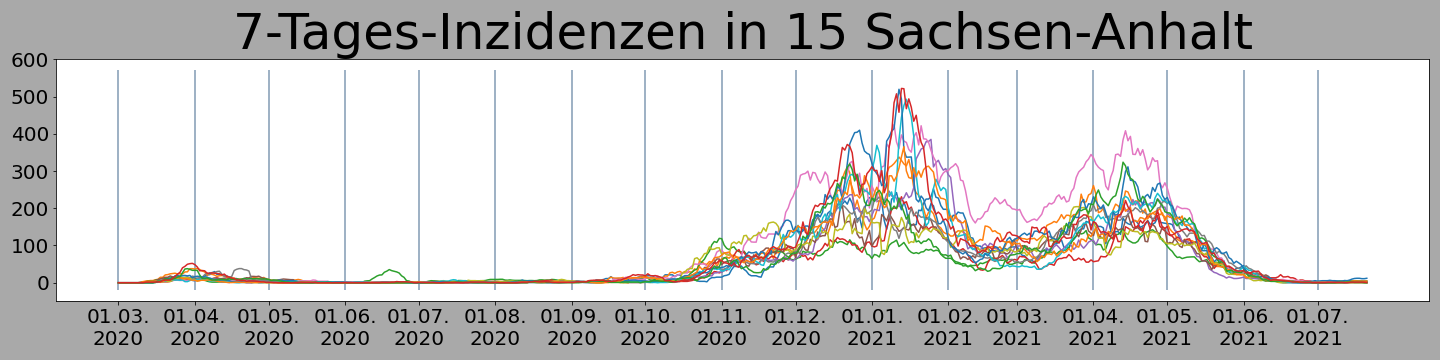
\includegraphics[width=\textwidth]{figures/Anhang/15_Sachsen-Anhalt.png}
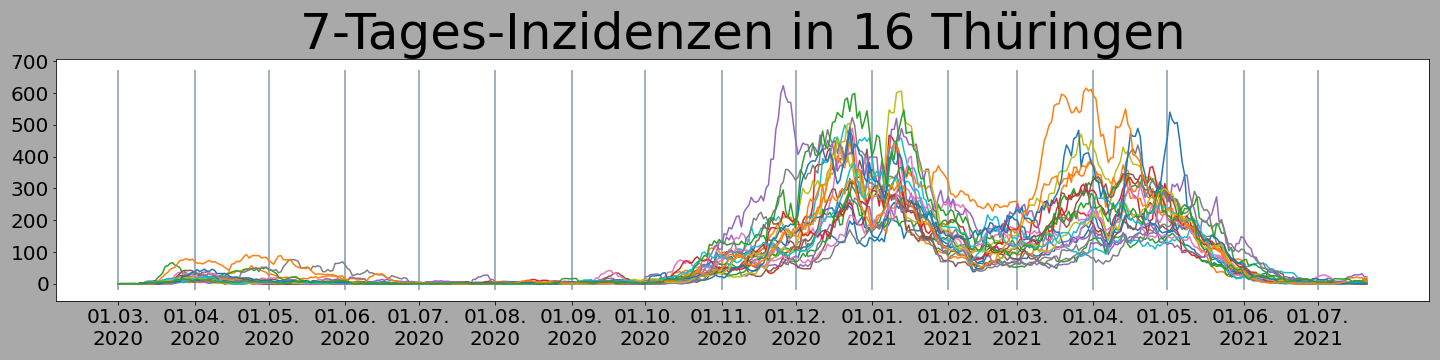
\includegraphics[width=\textwidth]{figures/Anhang/16_Thüringen.png}
\newpage
\begin{table}[H]
    \centering
    \begin{enumerate}[itemsep=-6mm]
\item 12070 LK Prignitz (35.60)
\item 15081 LK Altmarkkreis Salzwedel (36.11)
\item 12073 LK Uckermark (38.60)
\item 12068 LK Ostprignitz-Ruppin (39.11)
\item 3354 LK Lüchow-Dannenberg (39.48)
\item 13076 LK Ludwigslust-Parchim (44.43)
\item 15090 LK Stendal (45.62)
\item 13071 LK Mecklenburgische Seenplatte (46.92)
\item 12062 LK Elbe-Elster (53.50)
\item 15086 LK Jerichower Land (56.35)
\item 7232 LK Bitburg-Prüm (60.84)
\item 13075 LK Vorpommern-Greifswald (62.00)
\item 13072 LK Rostock (62.91)
\item 3360 LK Uelzen (63.21)
\item 15091 LK Wittenberg (64.26)
\item 9374 LK Neustadt a.d.Waldnaab (66.10)
\item 9377 LK Tirschenreuth (66.40)
\item 7233 LK Vulkaneifel (66.54)
\item 16069 LK Hildburghausen (67.42)
\item 12071 LK Spree-Neiße (68.45)
\item 16075 LK Saale-Orla-Kreis (69.73)
\item 13073 LK Vorpommern-Rügen (70.97)
\item 16065 LK Kyffhäuserkreis (71.52)
\item 15083 LK Börde (71.91)
\item 6535 LK Vogelsbergkreis (72.50)
\item 13074 LK Nordwestmecklenburg (74.06)
\item 3358 LK Heidekreis (74.80)
\item 12061 LK Dahme-Spreewald (74.91)
\item 9673 LK Rhön-Grabfeld (78.00)
\item 12067 LK Oder-Spree (79.03)
\item 3357 LK Rotenburg (Wümme) (79.04)
\item 9276 LK Regen (79.30)
\item 1054 LK Nordfriesland (79.47)
\item 9272 LK Freyung-Grafenau (79.49)
\item 9575 LK Neustadt a.d.Aisch-Bad Windsheim (79.71)
\item 12072 LK Teltow-Fläming (80.69)
\item 9472 LK Bayreuth (81.39)
\item 9371 LK Amberg-Sulzbach (82.09)
\item 12069 LK Potsdam-Mittelmark (83.45)
\item 9372 LK Cham (83.74)
\item 9278 LK Straubing-Bogen (84.12)
\item 6635 LK Waldeck-Frankenberg (84.71)
\item 16068 LK Sömmerda (86.06)
\item 3462 LK Wittmund (86.26)
\item 3256 LK Nienburg (Weser) (86.70)
\item 9180 LK Garmisch-Partenkirchen (87.40)
\item 9674 LK Haßberge (88.26)
\item 7135 LK Cochem-Zell (88.59)
\item 12066 LK Oberspreewald-Lausitz (89.24)
\item 12064 LK Märkisch-Oderland (90.52)
\item 9672 LK Bad Kissingen (90.80)
\item 16063 LK Wartburgkreis (91.14)
\item 15087 LK Mansfeld-Südharz (92.68)
\item 1051 LK Dithmarschen (93.44)
\item 9571 LK Ansbach (93.62)
\item 12063 LK Havelland (94.29)
\item 9277 LK Rottal-Inn (94.73)
\item 9677 LK Main-Spessart (95.51)
\item 3352 LK Cuxhaven (96.24)
\item 7231 LK Bernkastel-Wittlich (96.28)
\item 14730 LK Nordsachsen (97.44)
\item 9577 LK Weißenburg-Gunzenhausen (97.66)
\item 6636 LK Werra-Meißner-Kreis (98.30)
\item 7340 LK Südwestpfalz (99.44)
\item 16073 LK Saalfeld-Rudolstadt (99.59)
\item 9373 LK Neumarkt i.d.OPf. (100.08)
\item 1059 LK Schleswig-Flensburg (101.12)
\item 15085 LK Harz (101.23)
\item 9376 LK Schwandorf (101.34)
\item 9777 LK Ostallgäu (101.38)
\item 3255 LK Holzminden (101.53)
\item 8128 LK Main-Tauber-Kreis (101.53)
\item 16074 LK Saale-Holzland-Kreis (101.70)
\item 9780 LK Oberallgäu (102.13)
\item 16071 LK Weimarer Land (102.15)
\item 9476 LK Kronach (102.46)
\item 16066 LK Schmalkalden-Meiningen (103.22)
\item 7140 LK Rhein-Hunsrück-Kreis (104.13)
\item 7134 LK Birkenfeld (104.21)
\item 3155 LK Northeim (104.25)
\item 16064 LK Unstrut-Hainich-Kreis (104.46)
\item 9779 LK Donau-Ries (105.04)
\item 9475 LK Hof (106.08)
\item 16061 LK Eichsfeld (106.16)
\item 3461 LK Wesermarsch (107.00)
\item 15082 LK Anhalt-Bitterfeld (108.46)
\item 8437 LK Sigmaringen (108.71)
\item 9477 LK Kulmbach (108.76)
\item 3251 LK Diepholz (109.14)
\item 9176 LK Eichstätt (109.43)
\item 6632 LK Hersfeld-Rotenburg (110.04)
\item 9279 LK Dingolfing-Landau (110.09)
\item 3151 LK Gifhorn (112.55)
\item 3454 LK Emsland (113.43)
\item 16076 LK Greiz (115.05)
\item 9173 LK Bad Tölz-Wolfratshausen (115.06)
\item 9182 LK Miesbach (115.35)
\item 9273 LK Kelheim (115.54)
\item 3351 LK Celle (115.56)
\item 9189 LK Traunstein (115.56)
\item 6634 LK Schwalm-Eder-Kreis (116.79)
\item 16062 LK Nordhausen (116.84)
\item 5762 LK Höxter (116.89)
\item 7333 LK Donnersbergkreis (116.92)
\item 12065 LK Oberhavel (117.63)
\item 9778 LK Unterallgäu (118.24)
\item 9274 LK Landshut (118.60)
\item 1057 LK Plön (118.89)
\item 14626 LK Görlitz (119.33)
\item 9479 LK Wunsiedel i.Fichtelgebirge (119.82)
\item 3453 LK Cloppenburg (120.19)
\item 9773 LK Dillingen a.d.Donau (122.04)
\item 7336 LK Kusel (122.58)
\item 3458 LK Oldenburg (122.98)
\item 14625 LK Bautzen (124.81)
\item 12060 LK Barnim (124.88)
\item 9275 LK Passau (125.70)
\item 9172 LK Berchtesgadener Land (125.97)
\item 16070 LK Ilm-Kreis (126.01)
\item 15084 LK Burgenlandkreis (126.02)
\item 9471 LK Bamberg (126.15)
\item 1058 LK Rendsburg-Eckernförde (126.44)
\item 15088 LK Saalekreis (127.60)
\item 8225 LK Neckar-Odenwald-Kreis (127.72)
\item 9478 LK Lichtenfels (128.50)
\item 1061 LK Steinburg (128.78)
\item 9185 LK Neuburg-Schrobenhausen (131.50)
\item 15089 LK Salzlandkreis (131.77)
\item 5958 LK Hochsauerlandkreis (132.65)
\item 8127 LK Schwäbisch Hall (132.68)
\item 16072 LK Sonneberg (133.32)
\item 9675 LK Kitzingen (133.37)
\item 7235 LK Trier-Saarburg (135.17)
\item 3154 LK Helmstedt (135.17)
\item 8237 LK Freudenstadt (135.84)
\item 9678 LK Schweinfurt (137.29)
\item 9271 LK Deggendorf (138.55)
\item 3355 LK Lüneburg (138.82)
\item 9375 LK Regensburg (139.25)
\item 3456 LK Grafschaft Bentheim (139.72)
\item 9190 LK Weilheim-Schongau (140.07)
\item 3153 LK Goslar (140.74)
\item 9576 LK Roth (141.63)
\item 8426 LK Biberach (142.87)
\item 14522 LK Mittelsachsen (143.64)
\item 9183 LK Mühldorf a.Inn (143.83)
\item 16067 LK Gotha (144.19)
\item 1055 LK Ostholstein (144.71)
\item 8126 LK Hohenlohekreis (145.07)
\item 8425 LK Alb-Donau-Kreis (145.30)
\item 3452 LK Aurich (146.62)
\item 9473 LK Coburg (146.85)
\item 14628 LK Sächsische Schweiz-Osterzgebirge (148.19)
\item 9181 LK Landsberg a.Lech (149.75)
\item 8337 LK Waldshut (151.31)
\item 6437 LK Odenwaldkreis (154.88)
\item 5366 LK Euskirchen (154.93)
\item 14729 LK Leipzig (156.19)
\item 7141 LK Rhein-Lahn-Kreis (156.59)
\item 16077 LK Altenburger Land (156.89)
\item 1053 LK Herzogtum Lauenburg (156.90)
\item 9177 LK Erding (158.61)
\item 3455 LK Friesland (159.86)
\item 14523 LK Vogtlandkreis (159.94)
\item 3457 LK Leer (160.07)
\item 6631 LK Fulda (161.64)
\item 3158 LK Wolfenbüttel (165.26)
\item 7131 LK Ahrweiler (165.35)
\item 7335 LK Kaiserslautern (165.50)
\item 14627 LK Meißen (165.56)
\item 9774 LK Günzburg (166.46)
\item 9679 LK Würzburg (167.94)
\item 9186 LK Pfaffenhofen a.d.Ilm (168.55)
\item 3459 LK Osnabrück (168.94)
\item 3359 LK Stade (169.58)
\item 3451 LK Ammerland (171.21)
\item 9771 LK Aichach-Friedberg (172.72)
\item 7337 LK Südliche Weinstraße (172.92)
\item 3361 LK Verden (173.92)
\item 3356 LK Osterholz (174.55)
\item 8436 LK Ravensburg (175.02)
\item 3460 LK Vechta (175.60)
\item 9676 LK Miltenberg (180.13)
\item 9474 LK Forchheim (180.78)
\item 9187 LK Rosenheim (181.30)
\item 8325 LK Rottweil (181.89)
\item 10046 LK Sankt Wendel (182.70)
\item 6633 LK Kassel (182.92)
\item 14521 LK Erzgebirgskreis (183.13)
\item 7133 LK Bad Kreuznach (183.36)
\item 10042 LK Merzig-Wadern (185.42)
\item 3159 LK Göttingen (185.91)
\item 3252 LK Hameln-Pyrmont (186.33)
\item 5966 LK Olpe (188.36)
\item 8315 LK Breisgau-Hochschwarzwald (191.57)
\item 8327 LK Tuttlingen (191.93)
\item 9171 LK Altötting (195.65)
\item 6534 LK Marburg-Biedenkopf (195.93)
\item 5558 LK Coesfeld (198.41)
\item 8235 LK Calw (199.83)
\item 7132 LK Altenkirchen (201.01)
\item 3353 LK Harburg (203.83)
\item 7143 LK Westerwaldkreis (204.03)
\item 1060 LK Segeberg (206.07)
\item 8417 LK Zollernalbkreis (206.60)
\item 8326 LK Schwarzwald-Baar-Kreis (207.28)
\item 8136 LK Ostalbkreis (208.03)
\item 5570 LK Warendorf (210.84)
\item 8135 LK Heidenheim (211.76)
\item 9574 LK Nürnberger Land (214.11)
\item 7331 LK Alzey-Worms (220.71)
\item 7332 LK Bad Dürkheim (223.52)
\item 9178 LK Freising (225.41)
\item 5974 LK Soest (227.15)
\item 3254 LK Hildesheim (228.55)
\item 6439 LK Rheingau-Taunus-Kreis (230.66)
\item 8317 LK Ortenaukreis (231.89)
\item 6533 LK Limburg-Weilburg (232.80)
\item 3257 LK Schaumburg (233.54)
\item 9772 LK Augsburg (236.64)
\item 6532 LK Lahn-Dill-Kreis (237.96)
\item 9572 LK Erlangen-Höchstadt (243.24)
\item 5970 LK Siegen-Wittgenstein (244.38)
\item 8316 LK Emmendingen (244.71)
\item 5774 LK Paderborn (247.09)
\item 9671 LK Aschaffenburg (249.37)
\item 5566 LK Steinfurt (249.78)
\item 3157 LK Peine (251.49)
\item 5154 LK Kleve (253.32)
\item 9776 LK Lindau (253.85)
\item 9175 LK Ebersberg (261.16)
\item 5554 LK Borken (261.34)
\item 7137 LK Mayen-Koblenz (262.71)
\item 8415 LK Reutlingen (263.02)
\item 9174 LK Dachau (267.29)
\item 5770 LK Minden-Lübbecke (269.65)
\item 7334 LK Germersheim (278.61)
\item 5766 LK Lippe (279.17)
\item 6440 LK Wetteraukreis (280.31)
\item 9188 LK Starnberg (280.75)
\item 5358 LK Düren (281.41)
\item 8336 LK Lörrach (283.52)
\item 7138 LK Neuwied (291.39)
\item 5374 LK Oberbergischer Kreis (296.44)
\item 6435 LK Main-Kinzig-Kreis (301.30)
\item 8216 LK Rastatt (313.54)
\item 8125 LK Heilbronn (313.72)
\item 12051 SK Brandenburg a.d.Havel (314.58)
\item 6531 LK Gießen (316.70)
\item 1062 LK Stormarn (318.89)
\item 15001 SK Dessau-Roßlau (325.08)
\item 8435 LK Bodenseekreis (327.11)
\item 14524 LK Zwickau (331.45)
\item 10045 LK Saarpfalz-Kreis (339.44)
\item 9775 LK Neu-Ulm (339.97)
\item 8236 LK Enzkreis (348.34)
\item 7339 LK Mainz-Bingen (349.30)
\item 8335 LK Konstanz (350.57)
\item 16054 SK Suhl (359.18)
\item 6431 LK Bergstraße (376.28)
\item 5754 LK Gütersloh (376.70)
\item 9573 LK Fürth (383.80)
\item 5962 LK Märkischer Kreis (386.81)
\item 12053 SK Frankfurt (Oder) (389.89)
\item 8211 SK Baden-Baden (394.48)
\item 8117 LK Göppingen (402.00)
\item 16056 SK Eisenach (404.58)
\item 5370 LK Heinsberg (407.38)
\item 8215 LK Karlsruhe (410.76)
\item 9561 SK Ansbach (418.95)
\item 10044 LK Saarlouis (423.45)
\item 8416 LK Tübingen (440.13)
\item 5170 LK Wesel (441.33)
\item 3402 SK Emden (449.07)
\item 6432 LK Darmstadt-Dieburg (453.14)
\item 7316 SK Neustadt a.d.Weinstraße (454.29)
\item 3102 SK Salzgitter (463.65)
\item 7320 SK Zweibrücken (483.04)
\item 6434 LK Hochtaunuskreis (493.09)
\item 1056 LK Pinneberg (496.40)
\item 8119 LK Rems-Murr-Kreis (498.77)
\item 3241 Region Hannover (504.02)
\item 9179 LK Fürstenfeldbruck (504.63)
\item 7338 LK Rhein-Pfalz-Kreis (508.00)
\item 8226 LK Rhein-Neckar-Kreis (517.37)
\item 5382 LK Rhein-Sieg-Kreis (521.57)
\item 9184 LK München (527.71)
\item 10043 LK Neunkirchen (529.77)
\item 5166 LK Viersen (530.26)
\item 5758 LK Herford (556.29)
\item 7313 SK Landau i.d.Pfalz (565.34)
\item 12052 SK Cottbus (602.29)
\item 9363 SK Weiden i.d.OPf. (605.20)
\item 3103 SK Wolfsburg (606.93)
\item 6433 LK Groß-Gerau (608.61)
\item 16052 SK Gera (611.24)
\item 9764 SK Memmingen (631.64)
\item 8115 LK Böblingen (636.92)
\item 5378 LK Rheinisch-Bergischer Kreis (646.79)
\item 7317 SK Pirmasens (654.05)
\item 5362 LK Rhein-Erft-Kreis (669.34)
\item 9263 SK Straubing (705.98)
\item 3405 SK Wilhelmshaven (708.12)
\item 7312 SK Kaiserslautern (713.74)
\item 5978 LK Unna (727.94)
\item 13004 SK Schwerin (735.67)
\item 9262 SK Passau (750.62)
\item 7319 SK Worms (768.65)
\item 16055 SK Weimar (772.60)
\item 5162 LK Rhein-Kreis Neuss (783.40)
\item 9464 SK Hof (786.98)
\item 5954 LK Ennepe-Ruhr-Kreis (789.06)
\item 5334 StädteRegion Aachen (790.54)
\item 5915 SK Hamm (790.88)
\item 16051 SK Erfurt (791.77)
\item 8118 LK Ludwigsburg (794.77)
\item 10041 LK Stadtverband Saarbrücken (798.94)
\item 5562 LK Recklinghausen (806.93)
\item 9361 SK Amberg (836.63)
\item 8116 LK Esslingen (836.83)
\item 9463 SK Coburg (853.31)
\item 12054 SK Potsdam (963.50)
\item 7211 SK Trier (964.92)
\item 16053 SK Jena (969.41)
\item 6438 LK Offenbach (1000.03)
\item 9565 SK Schwabach (1007.16)
\item 1003 SK Lübeck (1022.93)
\item 9161 SK Ingolstadt (1028.17)
\item 5515 SK Münster (1039.25)
\item 8421 SK Ulm (1063.04)
\item 7111 SK Koblenz (1076.89)
\item 6436 LK Main-Taunus-Kreis (1077.20)
\item 9763 SK Kempten (1093.88)
\item 9762 SK Kaufbeuren (1098.03)
\item 9261 SK Landshut (1108.96)
\item 14511 SK Chemnitz (1112.67)
\item 7311 SK Frankenthal (1116.06)
\item 9462 SK Bayreuth (1116.14)
\item 1004 SK Neumünster (1123.16)
\item 9661 SK Aschaffenburg (1146.90)
\item 5512 SK Bottrop (1173.13)
\item 5914 SK Hagen (1177.24)
\item 7318 SK Speyer (1181.35)
\item 15003 SK Magdeburg (1184.71)
\item 5158 LK Mettmann (1190.65)
\item 13003 SK Rostock (1236.48)
\item 3401 SK Delmenhorst (1242.49)
\item 8121 SK Heilbronn (1258.60)
\item 8231 SK Pforzheim (1283.68)
\item 5711 SK Bielefeld (1290.85)
\item 3101 SK Braunschweig (1297.31)
\item 6411 SK Darmstadt (1299.31)
\item 6414 SK Wiesbaden (1367.95)
\item 3404 SK Osnabrück (1375.78)
\item 9461 SK Bamberg (1407.94)
\item 9562 SK Erlangen (1443.07)
\item 9663 SK Würzburg (1458.20)
\item 8221 SK Heidelberg (1478.74)
\item 4012 SK Bremerhaven (1483.07)
\item 8311 SK Freiburg i.Breisgau (1500.23)
\item 5120 SK Remscheid (1503.35)
\item 9662 SK Schweinfurt (1506.19)
\item 5116 SK Mönchengladbach (1528.98)
\item 11009 SK Berlin Treptow-Köpenick (1586.19)
\item 3403 SK Oldenburg (1631.36)
\item 5114 SK Krefeld (1664.19)
\item 14612 SK Dresden (1694.41)
\item 9163 SK Rosenheim (1727.63)
\item 4011 SK Bremen (1743.98)
\item 15002 SK Halle (1758.65)
\item 5122 SK Solingen (1789.94)
\item 8212 SK Karlsruhe (1794.67)
\item 1001 SK Flensburg (1833.24)
\item 5117 SK Mülheim a.d.Ruhr (1870.33)
\item 9362 SK Regensburg (1917.84)
\item 6611 SK Kassel (1936.46)
\item 14713 SK Leipzig (1982.44)
\item 9761 SK Augsburg (2025.77)
\item 9563 SK Fürth (2030.43)
\item 5316 SK Leverkusen (2078.83)
\item 5913 SK Dortmund (2104.24)
\item 5124 SK Wuppertal (2109.81)
\item 5112 SK Duisburg (2140.13)
\item 8222 SK Mannheim (2142.45)
\item 1002 SK Kiel (2198.97)
\item 7314 SK Ludwigshafen (2213.76)
\item 7315 SK Mainz (2238.90)
\item 5314 SK Bonn (2328.50)
\item 5513 SK Gelsenkirchen (2466.57)
\item 2000 SK Hamburg (2489.29)
\item 5911 SK Bochum (2525.55)
\item 11005 SK Berlin Spandau (2571.74)
\item 5315 SK Köln (2675.86)
\item 5119 SK Oberhausen (2720.89)
\item 9564 SK Nürnberg (2762.59)
\item 5113 SK Essen (2769.50)
\item 5111 SK Düsseldorf (2861.04)
\item 6413 SK Offenbach (2875.04)
\item 11012 SK Berlin Reinickendorf (2903.61)
\item 11006 SK Berlin Steglitz-Zehlendorf (2942.69)
\item 8111 SK Stuttgart (3033.65)
\item 5916 SK Herne (3039.06)
\item 6412 SK Frankfurt am Main (3077.83)
\item 11003 SK Berlin Pankow (3850.86)
\item 11010 SK Berlin Marzahn-Hellersdorf (4247.24)
\item 9162 SK München (4765.75)
\item 11004 SK Berlin Charlottenburg-Wilmersdorf (5162.54)
\item 11011 SK Berlin Lichtenberg (5489.14)
\item 11007 SK Berlin Tempelhof-Schöneberg (6433.60)
\item 11008 SK Berlin Neukölln (7136.56)
\item 11001 SK Berlin Mitte (9511.23)
\item 11002 SK Berlin Friedrichshain-Kreuzberg (13807.03)
\end{enumerate}
    \caption{Die deutschen Landkreise sortiert nach ihrer Bevölkerungsdichte.}
    \label{tab:counties_by_pop_density}
\end{table}
\newpage
\begin{table}[H]
    \centering
    \caption{Die deutschen Landkreise lexikographisch sortiert nach ihren Gemeindeschlüsseln.}
    \begin{tabular}{c c}
    1001&SK Flensburg\\ 
    1002&SK Kiel\\ 
    1003&SK Lübeck\\ 
    1004&SK Neumünster\\ 
    10041&LK Stadtverband Saarbrücken\\ 
    10042&LK Merzig-Wadern\\ 
    10043&LK Neunkirchen\\ 
    10044&LK Saarlouis\\ 
    10045&LK Saarpfalz-Kreis\\ 
    10046&LK Sankt Wendel\\ 
    1051&LK Dithmarschen\\ 
    1053&LK Herzogtum Lauenburg\\ 
    1054&LK Nordfriesland\\ 
    1055&LK Ostholstein\\ 
    1056&LK Pinneberg\\ 
    1057&LK Plön\\ 
    1058&LK Rendsburg-Eckernförde\\ 
    1059&LK Schleswig-Flensburg\\ 
    1060&LK Segeberg\\ 
    1061&LK Steinburg\\ 
    1062&LK Stormarn\\ 
    11001&SK Berlin Mitte\\ 
    11002&SK Berlin Friedrichshain-Kreuzberg\\ 
    11003&SK Berlin Pankow\\ 
    11004&SK Berlin Charlottenburg-Wilmersdorf\\ 
    11005&SK Berlin Spandau\\ 
    11006&SK Berlin Steglitz-Zehlendorf\\ 
    11007&SK Berlin Tempelhof-Schöneberg\\ 
    11008&SK Berlin Neukölln\\ 
    11009&SK Berlin Treptow-Köpenick\\ 
    11010&SK Berlin Marzahn-Hellersdorf\\ 
    11011&SK Berlin Lichtenberg\\ 
    11012&SK Berlin Reinickendorf\\ 
    12051&SK Brandenburg a.d.Havel\\ 
    12052&SK Cottbus\\ 
    12053&SK Frankfurt (Oder)\\ 
    12054&SK Potsdam\\ 
    12060&LK Barnim\\ 
    12061&LK Dahme-Spreewald\\ 
    12062&LK Elbe-Elster\\ 
    12063&LK Havelland\\ 
    12064&LK Märkisch-Oderland\\ 
    12065&LK Oberhavel\\ 
    12066&LK Oberspreewald-Lausitz\\ 
    12067&LK Oder-Spree\\ 
    12068&LK Ostprignitz-Ruppin\\ 
    12069&LK Potsdam-Mittelmark\\ 
    12070&LK Prignitz\\ 
    12071&LK Spree-Neiße\\ 
    12072&LK Teltow-Fläming\\ 
    12073&LK Uckermark\\ 
    13003&SK Rostock\\ 
    13004&SK Schwerin\\ 
    13071&LK Mecklenburgische Seenplatte\\ 
    13072&LK Rostock\\ 
    13073&LK Vorpommern-Rügen\\ 
    13074&LK Nordwestmecklenburg\\ 
    13075&LK Vorpommern-Greifswald\\ 
    13076&LK Ludwigslust-Parchim\\ 
    14511&SK Chemnitz\\ 
    14521&LK Erzgebirgskreis\\ 
    14522&LK Mittelsachsen\\ 
    14523&LK Vogtlandkreis\\ 
    14524&LK Zwickau\\ 
    14612&SK Dresden\\ 
    14625&LK Bautzen\\ 
    14626&LK Görlitz\\ 
    14627&LK Meißen\\ 
    14628&LK Sächsische Schweiz-Osterzgebirge\\ 
    14713&SK Leipzig\\ 
    14729&LK Leipzig\\ 
    14730&LK Nordsachsen\\ 
    15001&SK Dessau-Roßlau\\ 
    15002&SK Halle\\ 
    15003&SK Magdeburg\\ 
    15081&LK Altmarkkreis Salzwedel\\ 
    15082&LK Anhalt-Bitterfeld\\ 
    15083&LK Börde\\ 
    15084&LK Burgenlandkreis\\ 
    15085&LK Harz\\ 
    15086&LK Jerichower Land\\ 
    15087&LK Mansfeld-Südharz\\ 
    15088&LK Saalekreis\\ 
    15089&LK Salzlandkreis\\ 
    15090&LK Stendal\\ 
    15091&LK Wittenberg\\ 
    16051&SK Erfurt\\ 
    16052&SK Gera\\ 
    16053&SK Jena\\ 
    16054&SK Suhl\\ 
    16055&SK Weimar\\ 
    16056&SK Eisenach\\ 
    16061&LK Eichsfeld\\ 
    16062&LK Nordhausen\\ 
    16063&LK Wartburgkreis\\ 
    16064&LK Unstrut-Hainich-Kreis\\ 
    16065&LK Kyffhäuserkreis\\ 
    16066&LK Schmalkalden-Meiningen\\ 
    16067&LK Gotha\\ 
    16068&LK Sömmerda\\ 
    16069&LK Hildburghausen\\ 
    16070&LK Ilm-Kreis\\ 
    16071&LK Weimarer Land\\ 
    16072&LK Sonneberg\\ 
    16073&LK Saalfeld-Rudolstadt\\ 
    16074&LK Saale-Holzland-Kreis\\ 
    16075&LK Saale-Orla-Kreis\\ 
    16076&LK Greiz\\ 
    16077&LK Altenburger Land\\ 
    2000&SK Hamburg\\ 
    3101&SK Braunschweig\\ 
    3102&SK Salzgitter\\ 
    3103&SK Wolfsburg\\ 
    3151&LK Gifhorn\\ 
    3153&LK Goslar\\ 
    3154&LK Helmstedt\\ 
    3155&LK Northeim\\ 
    3157&LK Peine\\ 
    3158&LK Wolfenbüttel\\ 
    3159&LK Göttingen\\ 
    3241&Region Hannover\\ 
    3251&LK Diepholz\\ 
    3252&LK Hameln-Pyrmont\\ 
    3254&LK Hildesheim\\ 
    3255&LK Holzminden\\ 
    3256&LK Nienburg (Weser)\\ 
    3257&LK Schaumburg\\ 
    3351&LK Celle\\ 
    3352&LK Cuxhaven\\ 
    3353&LK Harburg\\ 
    3354&LK Lüchow-Dannenberg\\ 
    3355&LK Lüneburg\\ 
    3356&LK Osterholz\\ 
    3357&LK Rotenburg (Wümme)\\ 
    3358&LK Heidekreis\\ 
    3359&LK Stade\\ 
    3360&LK Uelzen\\ 
    3361&LK Verden\\ 
    3401&SK Delmenhorst\\ 
    3402&SK Emden\\ 
    3403&SK Oldenburg\\ 
    3404&SK Osnabrück\\ 
    3405&SK Wilhelmshaven\\ 
    3451&LK Ammerland\\ 
    3452&LK Aurich\\ 
    3453&LK Cloppenburg\\ 
    3454&LK Emsland\\ 
    3455&LK Friesland\\ 
    3456&LK Grafschaft Bentheim\\ 
    3457&LK Leer\\ 
    3458&LK Oldenburg\\ 
    3459&LK Osnabrück\\ 
    3460&LK Vechta\\ 
    3461&LK Wesermarsch\\ 
    3462&LK Wittmund\\ 
    4011&SK Bremen\\ 
    4012&SK Bremerhaven\\ 
    5111&SK Düsseldorf\\ 
    5112&SK Duisburg\\ 
    5113&SK Essen\\ 
    5114&SK Krefeld\\ 
    5116&SK Mönchengladbach\\ 
    5117&SK Mülheim a.d.Ruhr\\ 
    5119&SK Oberhausen\\ 
    5120&SK Remscheid\\ 
    5122&SK Solingen\\ 
    5124&SK Wuppertal\\ 
    5154&LK Kleve\\ 
    5158&LK Mettmann\\ 
    5162&LK Rhein-Kreis Neuss\\ 
    5166&LK Viersen\\ 
    5170&LK Wesel\\ 
    5314&SK Bonn\\ 
    5315&SK Köln\\ 
    5316&SK Leverkusen\\ 
    5334&StädteRegion Aachen\\ 
    5358&LK Düren\\ 
    5362&LK Rhein-Erft-Kreis\\ 
    5366&LK Euskirchen\\ 
    5370&LK Heinsberg\\ 
    5374&LK Oberbergischer Kreis\\ 
    5378&LK Rheinisch-Bergischer Kreis\\ 
    5382&LK Rhein-Sieg-Kreis\\ 
    5512&SK Bottrop\\ 
    5513&SK Gelsenkirchen\\ 
    5515&SK Münster\\ 
    5554&LK Borken\\ 
    5558&LK Coesfeld\\ 
    5562&LK Recklinghausen\\ 
    5566&LK Steinfurt\\ 
    5570&LK Warendorf\\ 
    5711&SK Bielefeld\\ 
    5754&LK Gütersloh\\ 
    5758&LK Herford\\ 
    5762&LK Höxter\\ 
    5766&LK Lippe\\ 
    5770&LK Minden-Lübbecke\\ 
    5774&LK Paderborn\\ 
    5911&SK Bochum\\ 
    5913&SK Dortmund\\ 
    5914&SK Hagen\\ 
    5915&SK Hamm\\ 
    5916&SK Herne\\ 
    5954&LK Ennepe-Ruhr-Kreis\\ 
    5958&LK Hochsauerlandkreis\\ 
    5962&LK Märkischer Kreis\\ 
    5966&LK Olpe\\ 
    5970&LK Siegen-Wittgenstein\\ 
    5974&LK Soest\\ 
    5978&LK Unna\\ 
    6411&SK Darmstadt\\ 
    6412&SK Frankfurt am Main\\ 
    6413&SK Offenbach\\ 
    6414&SK Wiesbaden\\ 
    6431&LK Bergstraße\\ 
    6432&LK Darmstadt-Dieburg\\ 
    6433&LK Groß-Gerau\\ 
    6434&LK Hochtaunuskreis\\ 
    6435&LK Main-Kinzig-Kreis\\ 
    6436&LK Main-Taunus-Kreis\\ 
    6437&LK Odenwaldkreis\\ 
    6438&LK Offenbach\\ 
    6439&LK Rheingau-Taunus-Kreis\\ 
    6440&LK Wetteraukreis\\ 
    6531&LK Gießen\\ 
    6532&LK Lahn-Dill-Kreis\\ 
    6533&LK Limburg-Weilburg\\ 
    6534&LK Marburg-Biedenkopf\\ 
    6535&LK Vogelsbergkreis\\ 
    6611&SK Kassel\\ 
    6631&LK Fulda\\ 
    6632&LK Hersfeld-Rotenburg\\ 
    6633&LK Kassel\\ 
    6634&LK Schwalm-Eder-Kreis\\ 
    6635&LK Waldeck-Frankenberg\\ 
    6636&LK Werra-Meißner-Kreis\\ 
    7111&SK Koblenz\\ 
    7131&LK Ahrweiler\\ 
    7132&LK Altenkirchen\\ 
    7133&LK Bad Kreuznach\\ 
    7134&LK Birkenfeld\\ 
    7135&LK Cochem-Zell\\ 
    7137&LK Mayen-Koblenz\\ 
    7138&LK Neuwied\\ 
    7140&LK Rhein-Hunsrück-Kreis\\ 
    7141&LK Rhein-Lahn-Kreis\\ 
    7143&LK Westerwaldkreis\\ 
    7211&SK Trier\\ 
    7231&LK Bernkastel-Wittlich\\ 
    7232&LK Bitburg-Prüm\\ 
    7233&LK Vulkaneifel\\ 
    7235&LK Trier-Saarburg\\ 
    7311&SK Frankenthal\\ 
    7312&SK Kaiserslautern\\ 
    7313&SK Landau i.d.Pfalz\\ 
    7314&SK Ludwigshafen\\ 
    7315&SK Mainz\\ 
    7316&SK Neustadt a.d.Weinstraße\\ 
    7317&SK Pirmasens\\ 
    7318&SK Speyer\\ 
    7319&SK Worms\\ 
    7320&SK Zweibrücken\\ 
    7331&LK Alzey-Worms\\ 
    7332&LK Bad Dürkheim\\ 
    7333&LK Donnersbergkreis\\ 
    7334&LK Germersheim\\ 
    7335&LK Kaiserslautern\\ 
    7336&LK Kusel\\ 
    7337&LK Südliche Weinstraße\\ 
    7338&LK Rhein-Pfalz-Kreis\\ 
    7339&LK Mainz-Bingen\\ 
    7340&LK Südwestpfalz\\ 
    8111&SK Stuttgart\\ 
    8115&LK Böblingen\\ 
    8116&LK Esslingen\\ 
    8117&LK Göppingen\\ 
    8118&LK Ludwigsburg\\ 
    8119&LK Rems-Murr-Kreis\\ 
    8121&SK Heilbronn\\ 
    8125&LK Heilbronn\\ 
    8126&LK Hohenlohekreis\\ 
    8127&LK Schwäbisch Hall\\ 
    8128&LK Main-Tauber-Kreis\\ 
    8135&LK Heidenheim\\ 
    8136&LK Ostalbkreis\\ 
    8211&SK Baden-Baden\\ 
    8212&SK Karlsruhe\\ 
    8215&LK Karlsruhe\\ 
    8216&LK Rastatt\\ 
    8221&SK Heidelberg\\ 
    8222&SK Mannheim\\ 
    8225&LK Neckar-Odenwald-Kreis\\ 
    8226&LK Rhein-Neckar-Kreis\\ 
    8231&SK Pforzheim\\ 
    8235&LK Calw\\ 
    8236&LK Enzkreis\\ 
    8237&LK Freudenstadt\\ 
    8311&SK Freiburg i.Breisgau\\ 
    8315&LK Breisgau-Hochschwarzwald\\ 
    8316&LK Emmendingen\\ 
    8317&LK Ortenaukreis\\ 
    8325&LK Rottweil\\ 
    8326&LK Schwarzwald-Baar-Kreis\\ 
    8327&LK Tuttlingen\\ 
    8335&LK Konstanz\\ 
    8336&LK Lörrach\\ 
    8337&LK Waldshut\\ 
    8415&LK Reutlingen\\ 
    8416&LK Tübingen\\ 
    8417&LK Zollernalbkreis\\ 
    8421&SK Ulm\\ 
    8425&LK Alb-Donau-Kreis\\ 
    8426&LK Biberach\\ 
    8435&LK Bodenseekreis\\ 
    8436&LK Ravensburg\\ 
    8437&LK Sigmaringen\\ 
    9161&SK Ingolstadt\\ 
    9162&SK München\\ 
    9163&SK Rosenheim\\ 
    9171&LK Altötting\\ 
    9172&LK Berchtesgadener Land\\ 
    9173&LK Bad Tölz-Wolfratshausen\\ 
    9174&LK Dachau\\ 
    9175&LK Ebersberg\\ 
    9176&LK Eichstätt\\ 
    9177&LK Erding\\ 
    9178&LK Freising\\ 
    9179&LK Fürstenfeldbruck\\ 
    9180&LK Garmisch-Partenkirchen\\ 
    9181&LK Landsberg a.Lech\\ 
    9182&LK Miesbach\\ 
    9183&LK Mühldorf a.Inn\\ 
    9184&LK München\\ 
    9185&LK Neuburg-Schrobenhausen\\ 
    9186&LK Pfaffenhofen a.d.Ilm\\ 
    9187&LK Rosenheim\\ 
    9188&LK Starnberg\\ 
    9189&LK Traunstein\\ 
    9190&LK Weilheim-Schongau\\ 
    9261&SK Landshut\\ 
    9262&SK Passau\\ 
    9263&SK Straubing\\ 
    9271&LK Deggendorf\\ 
    9272&LK Freyung-Grafenau\\ 
    9273&LK Kelheim\\ 
    9274&LK Landshut\\ 
    9275&LK Passau\\ 
    9276&LK Regen\\ 
    9277&LK Rottal-Inn\\ 
    9278&LK Straubing-Bogen\\ 
    9279&LK Dingolfing-Landau\\ 
    9361&SK Amberg\\ 
    9362&SK Regensburg\\ 
    9363&SK Weiden i.d.OPf.\\ 
    9371&LK Amberg-Sulzbach\\ 
    9372&LK Cham\\ 
    9373&LK Neumarkt i.d.OPf.\\ 
    9374&LK Neustadt a.d.Waldnaab\\ 
    9375&LK Regensburg\\ 
    9376&LK Schwandorf\\ 
    9377&LK Tirschenreuth\\ 
    9461&SK Bamberg\\ 
    9462&SK Bayreuth\\ 
    9463&SK Coburg\\ 
    9464&SK Hof\\ 
    9471&LK Bamberg\\ 
    9472&LK Bayreuth\\ 
    9473&LK Coburg\\ 
    9474&LK Forchheim\\ 
    9475&LK Hof\\ 
    9476&LK Kronach\\ 
    9477&LK Kulmbach\\ 
    9478&LK Lichtenfels\\ 
    9479&LK Wunsiedel i.Fichtelgebirge\\ 
    9561&SK Ansbach\\ 
    9562&SK Erlangen\\ 
    9563&SK Fürth\\ 
    9564&SK Nürnberg\\ 
    9565&SK Schwabach\\ 
    9571&LK Ansbach\\ 
    9572&LK Erlangen-Höchstadt\\ 
    9573&LK Fürth\\ 
    9574&LK Nürnberger Land\\ 
    9575&LK Neustadt a.d.Aisch-Bad Windsheim\\ 
    9576&LK Roth\\ 
    9577&LK Weißenburg-Gunzenhausen\\ 
    9661&SK Aschaffenburg\\ 
    9662&SK Schweinfurt\\ 
    9663&SK Würzburg\\ 
    9671&LK Aschaffenburg\\ 
    9672&LK Bad Kissingen\\ 
    9673&LK Rhön-Grabfeld\\ 
    9674&LK Haßberge\\ 
    9675&LK Kitzingen\\ 
    9676&LK Miltenberg\\ 
    9677&LK Main-Spessart\\ 
    9678&LK Schweinfurt\\ 
    9679&LK Würzburg\\ 
    9761&SK Augsburg\\ 
    9762&SK Kaufbeuren\\ 
    9763&SK Kempten\\ 
    9764&SK Memmingen\\ 
    9771&LK Aichach-Friedberg\\ 
    9772&LK Augsburg\\ 
    9773&LK Dillingen a.d.Donau\\ 
    9774&LK Günzburg\\ 
    9775&LK Neu-Ulm\\ 
    9776&LK Lindau\\ 
    9777&LK Ostallgäu\\ 
    9778&LK Unterallgäu\\ 
    9779&LK Donau-Ries\\ 
    9780&LK Oberallgäu\\ 

\end{tabular}
    \label{tab:counties_by_admunitid}
\end{table}
\newpage
\begin{table}[H]
    \centering
    13  Mecklenburg-Vorpommern

12  Brandenburg

15  Sachsen-Anhalt

72  Trier

33  L�neburg

93  Oberpfalz

92  Niederbayern

16  Th�ringen

66  Kassel

94  Oberfranken

96  Unterfranken

34  Weser-Ems

71  Koblenz

1  Schleswig-Holstein

97  Schwaben

65  Gie�en

31  Braunschweig

146  Dresden

84  T�bingen

145  Chemnitz

32  Hannover

83  Freiburg

95  Mittelfranken

147  Leipzig

91  Oberbayern

73  Rheinhessen-Pfalz

57  Detmold

55  M�nster

10  Saarland

81  Stuttgart

82  Karlsruhe

59  Arnsberg

64  Darmstadt

53  K�ln

51  D�sseldorf

4  Bremen

2  Hamburg

11  Berlin


    \caption{Die Regierungsbezirke sortiert nach ihrer Bevölkerungsdichte.}
    \label{tab:districts_by_pop_density}
\end{table}
\newpage
\begin{table}[H]
    \centering
    1  Schleswig-Holstein

10  Saarland

11  Berlin

12  Brandenburg

13  Mecklenburg-Vorpommern

145  Chemnitz

146  Dresden

147  Leipzig

15  Sachsen-Anhalt

16  Thüringen

2  Hamburg

31  Braunschweig

32  Hannover

33  Lüneburg

34  Weser-Ems

4  Bremen

51  Düsseldorf

53  Köln

55  Münster

57  Detmold

59  Arnsberg

64  Darmstadt

65  Gießen

66  Kassel

71  Koblenz

72  Trier

73  Rheinhessen-Pfalz

81  Stuttgart

82  Karlsruhe

83  Freiburg

84  Tübingen

91  Oberbayern

92  Niederbayern

93  Oberpfalz

94  Oberfranken

95  Mittelfranken

96  Unterfranken

97  Schwaben


    \caption{Die Regierungsbezirke lexikographisch sortiert nach den ersten beiden Teilen der Gemeindeschlüssel ihrer Landkreise.}
    \label{tab:districts_by_admunitid}
\end{table}
\newpage
